\documentclass[12pt]{article}

\usepackage{color}
\usepackage{graphicx}
\usepackage{amsmath}
\usepackage{float}
\usepackage{color}
\usepackage{indentfirst}
\usepackage{textcomp}
\usepackage{pifont}
\usepackage{multirow}
\usepackage{geometry}
\usepackage{algorithm}
\usepackage{algpseudocode}
\usepackage{amssymb}
\usepackage{algorithmicx}
\usepackage{amsmath} 
\usepackage{amsfonts}

\geometry{left = 2cm, right = 2cm, top = 3cm, bottom = 3cm}



\floatname{algorithm}{Algorithm}
\renewcommand{\algorithmicrequire}{\textbf{Input:}}
\renewcommand{\algorithmicensure}{\textbf{Output:}}





\begin{document}

\vspace*{0.25cm}

\hrulefill

\thispagestyle{empty}

\begin{center}
\begin{large}
\sc{UM--SJTU Joint Institute \vspace{0.3em} \\ Bayesian Analysis \\ (VE414)}
\end{large}

\hrulefill

\vspace*{5cm}
\begin{Large}
\sc{{Class Notes \\ ~\\ Class 2 Inference}}
\end{Large}
\vspace{2em}

\end{center}


\vfill
\begin{large}

\begin{table}[h!]
\flushleft
\begin{tabular}{lll}
Name: Wu Guangzheng \hspace*{2em}&

\end{tabular}
\end{table}
\end{large}
\newpage
\begin{flushleft}


\section{Basic Information}

\qquad Thomas Bayesian's origin problem: Given the number of times in which an unknown event has happened and failed: Required the chance that the probability of its happening in a single trial lies somewhere between any two degrees of probability that can be named.”

~\\

\qquad It is about statistical inference on binomial proportion $p$:

$$X \sim \text{Binominal}(k,p)$$

~\\

\textbf{A Ball Game Example}[H]

\qquad Suppose we have a black ball and a red ball. We first throw the black ball on the table, but we don't know where the black ball locates. Then we throw the red ball on the table, and we can know whether the red ball is farther or closer. Our aim is to find out where exactly the black ball locates.

\begin{figure}[H]
\centering
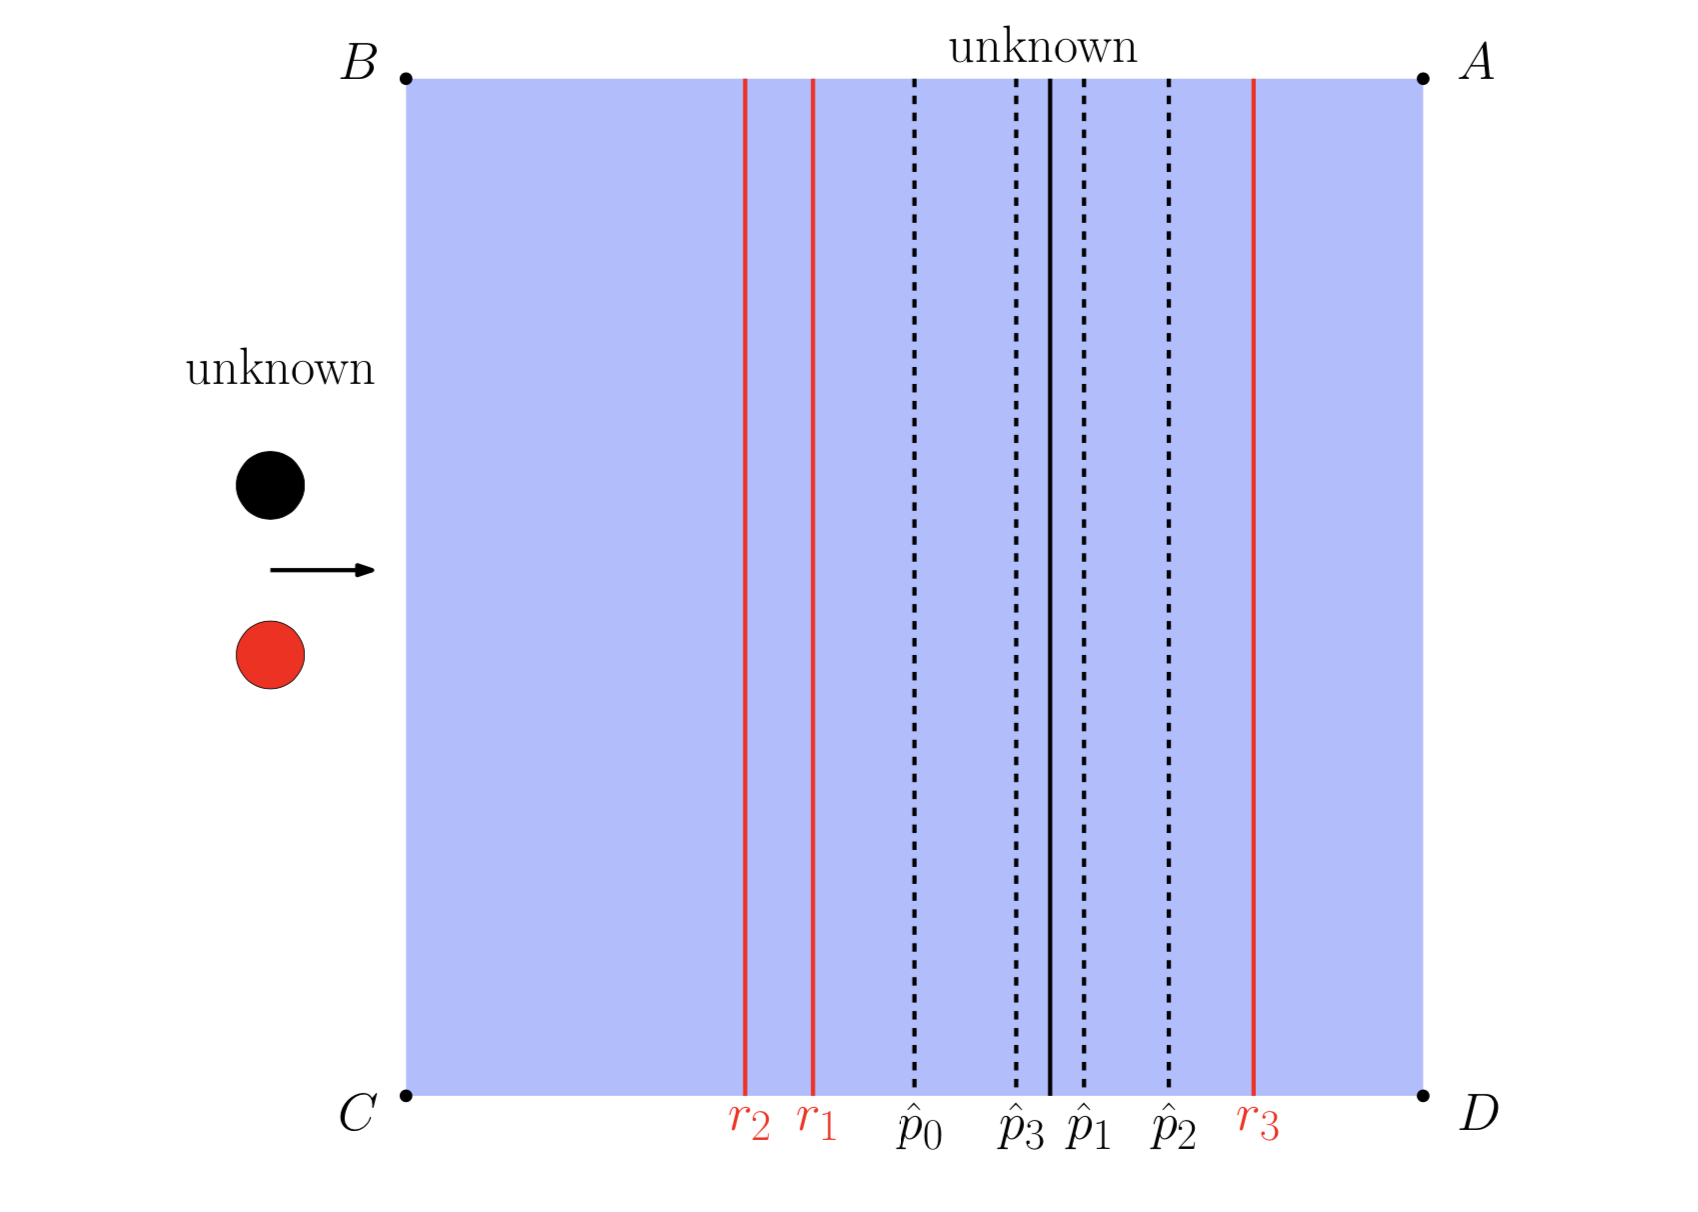
\includegraphics[width = 0.7\textwidth]{ball-game.png}
\caption{Ball Game Example}
\end{figure}

\section{Maximum Likelihood Estimator}

\qquad Since each throw of red ball is independent, we can assume that the result should follows the binominal distribution.

$$X \sim \text{Binominal}(k,p)$$

\qquad Then the likelihood of this should be 

$$L(p;x) = f_{X\mid p}(x\mid p) = \frac{k!}{x!(k-x)!}p^{x}(1-p)^{k-x}$$

\qquad A very arrogant way of solving this problem is named Maximum Likelihood Estimate, where we try to maximize the likelihood. It is one of typical frequentist solutions.

$$\tilde{\theta}_{MLE} = \mathop{\text{argmax}}\limits_{\theta \in \Theta} L(\theta; x)$$

\qquad And for this ball game, we can conclude that the Estimator should be 

$$\tilde{p} = \frac{x}{k}, \quad x\text{ for number of success, } k\text{ for number of trials}$$

\qquad As we mentioned above, the maximum likelihood estimate is an arrogant approach, where one can get some results far from the real value when the trial is small. Consider the case where one throw the black ball to the middle, and only throw one trial of read ball. In this case, the maximum likelihood estimate will have an estimator either to be 0, or be 1, which are both far from the actual result.

\section{Probability Mass Function and Probability Density Function}

\qquad Recall that for a discrete random variable, its PMF(probability mass function) is

$$f_{Y\mid X}(y\mid x) = \frac{f_{X,Y}(x, y)}{f_{X}(x)}, \qquad f_{X}(x) \neq 0$$

\qquad It is meaningful because PMF gives probability directly by

$$f_{Y\mid X}(y\mid x) = \text{Pr}(Y = y \mid X = x) = \frac{Pr(X = x, Y = y)}{Pr(X = x)} = \frac{f_{X,Y}(x, y)}{f_{X}(x)}$$

\qquad However, for a continuous random variable $x$, PDF does not link to probability directly

$$f_{Y\mid X}(y\mid x) \neq \text{Pr}(Y = y \mid X = x)$$

\qquad What's more, for any continuous random variable $x_c$ here, we always have

$$\text{Pr}(c) = 0$$

\section{Some Generally Used Distributions}

\subsection*{Binominal Distribution} 

\qquad Distribution: 

$$X \sim \text{Binominal}(k,p)$$

\qquad Probability Mass Function: 

$$f_{X}(x) = \frac{k!}{x!(k-x)!}p^x(1-p)^{k-x}$$ 

\qquad Support\footnote{Support: The possible values for random variable x}: 

$$x \in \{0, 1, 2, \cdots, k \}$$

\qquad Mean and Variance: 

$$\mathbb{E}(x) = kp\qquad \qquad \text{Var}(x) = kp(1-p)$$

\subsection*{Geometric Distribution} 

\qquad Distribution: 

$$X \sim \text{Geometric}(p)$$

\qquad Probability Mass Function: 

$$f_{X}(x) = p(1-p)^{x-1}$$ 

\qquad Support: 

$$x \in \{1, 2, \cdots, k \}$$

\qquad Mean: 

$$\mathbb{E}(x) = \frac{1}{p}$$

\qquad Variance: 

$$\text{Var}(x) = \frac{1-p}{p^2}$$


\section{Quiz}


\end{flushleft}
\end{document}